\documentclass[10pt, xcolor=svgnames]{beamer}

\usepackage[T1]{fontenc}
\usepackage[utf8]{inputenc}
\usepackage{hyperref}
\usepackage{siunitx}
\usepackage{tikz}
\usepackage[european]{circuitikz}
\usepackage{verbatim}

\usepackage{bookmark}

\usetheme{Pittsburgh}
\usecolortheme{dove}

\title{Lattice Watering: Final Results}

\author{Christian Müller, Jonas Heinemann, Kaan Dönmez, Valentin Pickel}

\institute{
    Software Project on Internet Communication

    Summer Term 2022
    
    Freie Universität Berlin

    Institute for Computer Science
}

\date{July 18, 2022}

\begin{document}

\maketitle

\begin{frame}{The Idea}

    \includegraphics[angle=90, width=0.4\linewidth]{img/IMG_20220711_154353_966.jpg}

\end{frame}

\begin{frame}{Goals}

    \begin{itemize}
        \item Develop a small but secure system for controlling several devices that can regularly water plants.
        \item Learn about techniques and challenges in developing IoT-based systems.
        \item Learn about RIOT.
    \end{itemize}

    Especially: With respect to the rough split we set at the beginning of the lecture, we worked in the world of the Internet of Things.

    \phantom{}

    We will look at the hardware deployed, the way we designed the communication between devices and our development process.
\end{frame}

\begin{frame}
    \frametitle{Hardware Overview}

    We differentiate between three types of devices: A \emph{host}, a \emph{border router} and \emph{nodes}. The hardware used (for references see the file mentioned below):

    \begin{enumerate}
        \item One personal computer with the software set up.
        \item Two SAMR21-XPRO boards (class 2 devices according to RFC 7228), one border router and one node.
        \item Two micro USB cables, optionally a battery connector or powerbank.
        \item One DRV8833 motor driver board.
        \item One electronic pump. It should come with a long tube.
        \item One capacitive moisture sensor.
        \item Nine female jumper cables.
        \item Five male jumper cables.
    \end{enumerate}

    The \texttt{HWSETUP.md} file describes how to put a node together.    

    The biggest problem we encountered was the following: The pump needs more current than any other component, about \qty{200}{\milli\ampere}. But a GPIO pin on our board can only handle \qty{92}{\milli\ampere}! We may destroy the board by directly connecting everything.
\end{frame}

\begin{frame}
    \frametitle{Hardware Overview}

    Initial attempts at fixing the problem with the current. involved this design, sadly the transistor given by Hauke did not work, so he got us some predesigned motor boards for assistence.

    \begin{figure}[htbp!]
        \centering
        \resizebox{0.75\linewidth}{5cm}{%
        \begin{circuitikz}
            \ctikzset{multipoles/dipchip/width=3}
            \draw (0, 0) node[dipchip, num pins=24, hide numbers, draw only pins={15, 23, 24}, no topmark] (B) {\texttt{SAMR21-XPRO}};
            \draw (B.bpin 24) circle[radius=1.5pt];
            \draw (B.bpin 23) circle[radius=1.5pt];
            \draw (B.bpin 15) circle[radius=1.5pt];
            \node [left] at (B.bpin 24) {\texttt{5V0}};
            \node [left] at (B.bpin 23) {\texttt{GND}};
            \node [left] at (B.bpin 15) {\texttt{PB03}};
            \draw (B.bpin 24) -- +(7, 0) node[above, pos=0.5] {5V};
            \draw ($(B.bpin 24)+(7, 0)$) circle[radius=1.5pt];
            \draw (B.bpin 23) -- +(2, 0);
            \draw ($(B.bpin 24)+(7, -4)$) node[nigfete, bodydiode, tr circle] (mos) {}
                (mos.source) node[anchor=north, below right] {\texttt{S}}
                (mos.gate) node[anchor=east, above left]     {\texttt{G}}
                (mos.drain) node[anchor=south, above right]  {\texttt{D}};
            \draw (mos.source) -- +(0, -2);
            \draw ($(mos.source)+(0, -2)$) -- ($(mos.source)+(-2, -2)$);
            \draw ($(mos.source)+(-2, -2)$) circle[radius=1.5pt];
            \draw (mos.gate) -- +(-1, 0);
            \draw ($(mos.gate)+(-1, 0)$) circle[radius=1.5pt];
            \draw ($(mos.source)+(-2, -2)$) -- ($(mos.source)+(-5, -2)$) -- ($(B.bpin 23)+(2, 0)$);
            \draw ($(mos.gate)+(-3.5, 0)$) to[R=\qty{200}{\ohm}] ($(mos.gate)+(-1, 0)$);
            \draw ($(mos.gate)+(-1, 0)$) to[R=\qty{5}{\kilo\ohm}] ($(mos.source)+(-2, -2)$);
            \draw ($(mos.gate)+(-3.5, 0)$) -- ($(mos.gate)+(-3.5, -0.775)$) -- (B.bpin 15);
            \draw ($(B.bpin 24)+(7, 0)$) -- +(0, -1);
            \draw ($(B.bpin 24)+(7, -1.5)$) circle[radius=0.5];
            \node at ($(B.bpin 24)+(7, -1.5)$) {\texttt{P}};
            \draw ($(B.bpin 24)+(7, -2)$) -- (mos.source);
        \end{circuitikz}
        }
    \end{figure}
\end{frame}

\begin{frame}
    \frametitle{Software Architecture}

    We developed two firmwares and two softwares in total. We list them with the programming languages used:

    \begin{itemize}
        \item \texttt{fw} (C, Makefile): This firmware runs on every board and controls the sensory, as well as the pumps. It uses SixLoWPAN and CoAP with DTLS to send the sensor data to the host.
        \item \texttt{br} (C, Makefile): A border router based on RIOTOS. It translates the SixLoWPAN traffic and routes it to the computer over a USB cable. It also uses \texttt{ethos} (Ethernet over Serial), a small technology developed by the RIOTOS project.
        \item \texttt{proxy} (Rust): Translates DTLS traffic to UDP traffic. Thus, we have transport security in the SixLoWPAN network.
        \item \texttt{front} (JS, HTML, CSS, SQL): The frontend has two parts: A node.js backend and a website. The backend stores the sensor data in a SQLite database, and the website allows the user to manually start pumps, look at humidity data over time, calibrate sensory and more.
    \end{itemize}
\end{frame}

\begin{frame}[fragile]
    \frametitle{Network Structure}
    \begin{figure}[!hbtp]
        \centering
        \resizebox{0.75\linewidth}{6cm}{%
        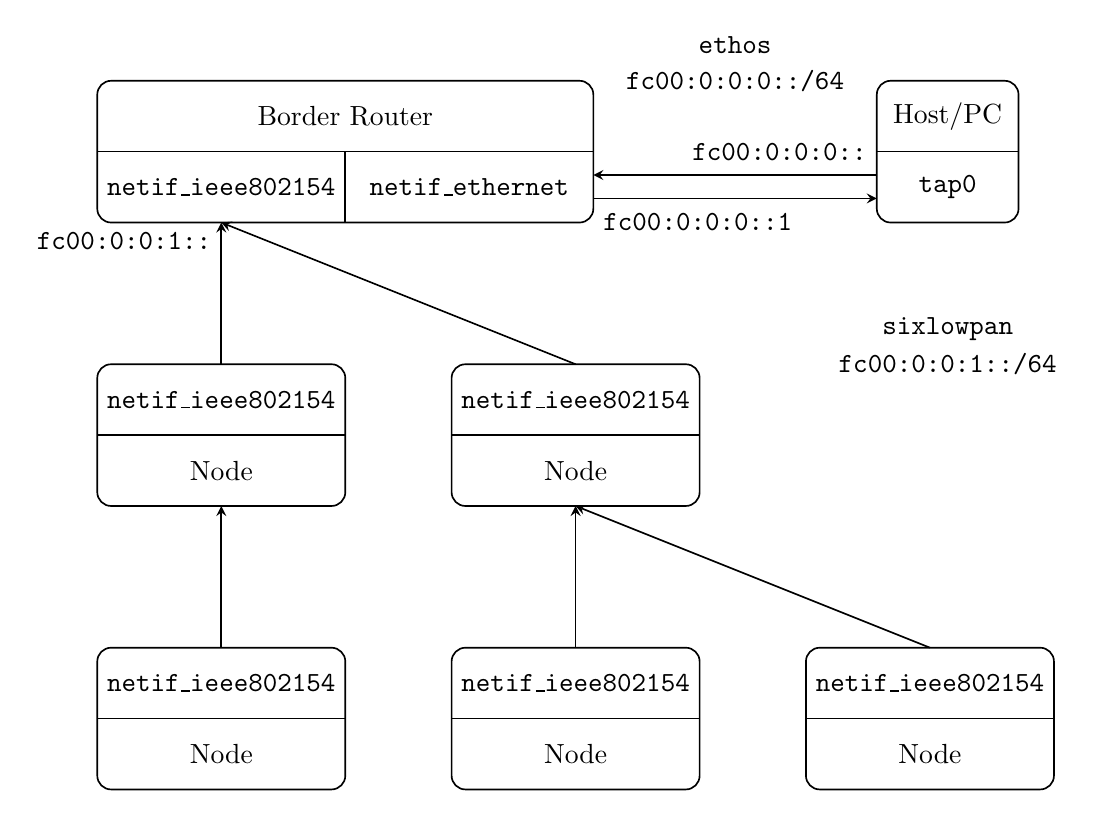
\begin{tikzpicture}[>=stealth, semithick, scale=0.9]
            \draw[rounded corners=5pt] (-1, -1) rectangle (1, 1);
            \draw[draw=none] (-1, 0) -- (1, 1) node[pos=0.5] {Host/PC};
            \draw (-1, 0) -- (1, 0);
            \draw[draw=none] (-1, 0) -- (1, -1) node[pos=0.5] {\texttt{tap0}};

            \draw[rounded corners=5pt] (-12, -1) rectangle (-5, 1);
            \draw[draw=none] (-12, 0) -- (-5, 1) node[pos=0.5] {Border Router};
            \draw (-12, 0) -- (-5, 0);
            \draw (-8.5, 0) -- (-8.5, -1);
            \draw[draw=none] (-12, 0) -- (-8.5, -1) node[pos=0.5] {\texttt{netif\_ieee802154}};
            \draw[draw=none] (-8.5, 0) -- (-5, -1) node[pos=0.5] {\texttt{netif\_ethernet}};
            \draw[->] (-1, -0.33) -- (-5, -0.33);
            \node[left] at (-1, 0) {\texttt{fc00:0:0:0::}};
            \node[right] at (-5, -1) {\texttt{fc00:0:0:0::1}};
            \node at (-3, 1.5) {\texttt{ethos}};
            \node at (-3, 1) {\texttt{fc00:0:0:0::/64}};
            \draw[->] (-5, -0.66) -- (-1, -0.66);
            \node[below left] at (-12+1.75, -1) {\texttt{fc00:0:0:1::}};

            \newcommand{\networknode}[2]{
                \draw[rounded corners=5pt] (#1, #2) rectangle (#1+3.5, #2-2);
                \draw (#1, #2-1) -- (#1+3.5, #2-1);
                \draw[draw=none] (#1, #2) -- (#1+3.5, #2-1) node[pos=0.5] {\texttt{netif\_ieee802154}};
                \draw[draw=none] (#1, #2-1) -- (#1+3.5, #2-2) node[pos=0.5] {Node};
            }

            \networknode{-12}{-3};
            \networknode{-7}{-3};
            \networknode{-12}{-7};
            \networknode{-7}{-7};
            \networknode{-2}{-7};

            \draw[->] (-12+1.75, -3) -- (-12+1.75, -1);
            \draw[->] (-7+1.75, -3) -- (-12+1.75, -1);
            \draw[->] (-12+1.75, -7) -- (-12+1.75, -5);
            \draw[->] (-7+1.75, -7) -- (-7+1.75, -5);
            \draw[->] (-2+1.75, -7) -- (-7+1.75, -5);

            \node at (0, -2.5) {\texttt{sixlowpan}};
            \node at (0, -3) {\texttt{fc00:0:0:1::/64}};
        \end{tikzpicture}
        }
    \end{figure}
\end{frame}

\begin{frame}
    \frametitle{Proxy}

    \begin{figure}[!hbtp]
        \centering
        \resizebox{\linewidth}{2.5cm}{%
        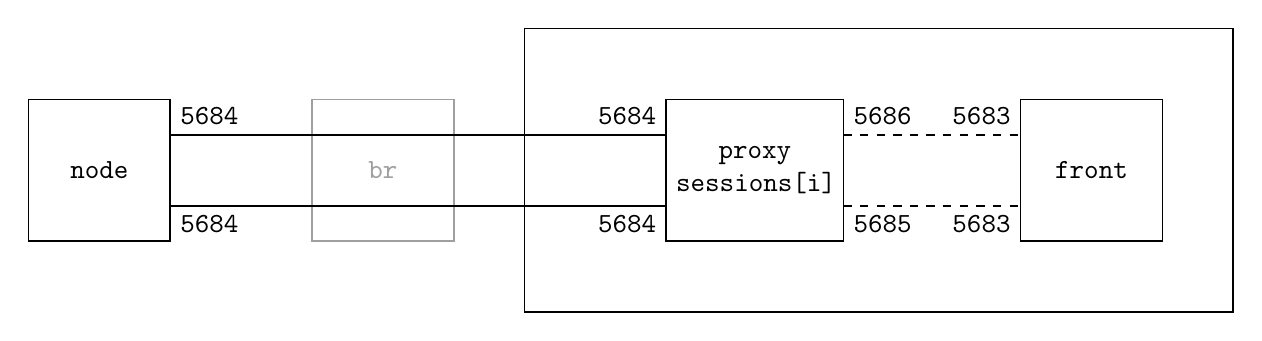
\begin{tikzpicture}[>=stealth, semithick, scale=0.9]
            \draw (0, 0) rectangle (2, -2) node[pos=0.5] {\texttt{node}};
            \draw[draw=gray!75] (4, 0) rectangle (4+2, -2) node[pos=0.5] {\textcolor{gray!75}{\texttt{br}}};
            \draw (7, 1) rectangle (8+9, -3) node[pos=0.5] {};
            \draw (9, 0) rectangle (9+2.5, -2) node[align=center, pos=0.5, text width=2cm] {
                \texttt{proxy}\\
                \texttt{sessions[i]}
            };
            \draw (14, 0) rectangle (14+2, -2) node[pos=0.5] {\texttt{front}};
            \draw (2, -0.5) -- (9, -0.5);
            \node[above right] at (2, -0.5) {\texttt{5684}};
            \node[above left] at (9, -0.5) {\texttt{5684}};
            \draw (2, -1.5) -- (9, -1.5);
            \node[below right] at (2, -1.5) {\texttt{5684}};
            \node[below left] at (9, -1.5) {\texttt{5684}};
            \node[above right] at (11.5, -0.5) {\texttt{5686}};
            \node[below right] at (11.5, -1.5) {\texttt{5685}};
            \node[above left] at (14, -0.5) {\texttt{5683}};
            \node[below left] at (14, -1.5) {\texttt{5683}};
            \draw[dashed] (11.5, -0.5) -- (14, -0.5);
            \draw[dashed] (11.5, -1.5) -- (14, -1.5);
        \end{tikzpicture}
        }
    \end{figure}
\end{frame}

\begin{frame}
    \frametitle{Communication Protocols Involved}

    \begin{itemize}
        \item All communication is based on IPv6 in the lower parts. We do not use any IPv4 addresses.
        \item The nodes, together with the border router, form a DODAG structure due to the RPL protocol. They also use SixLoWPAN to compress and fragment their IPv6 packets, such that if one places many around a huge house, they can route in a lossy network.
        \item The nodes indirectly talk with the DTLS proxy running on the hosts computer, which decrypts their traffic to forward the packets to the frontend.
        \item Notice that the finer details show up when looking closely: For the devices to find each others local address, IPv6 uses neighbor and router solicitation messages, and the DTLS protocol must establish a secure session before sending encrypted packets. So snooped traffic looks more complicated than expected.
    \end{itemize}

\end{frame}

\begin{frame}
    \frametitle{Demo}

    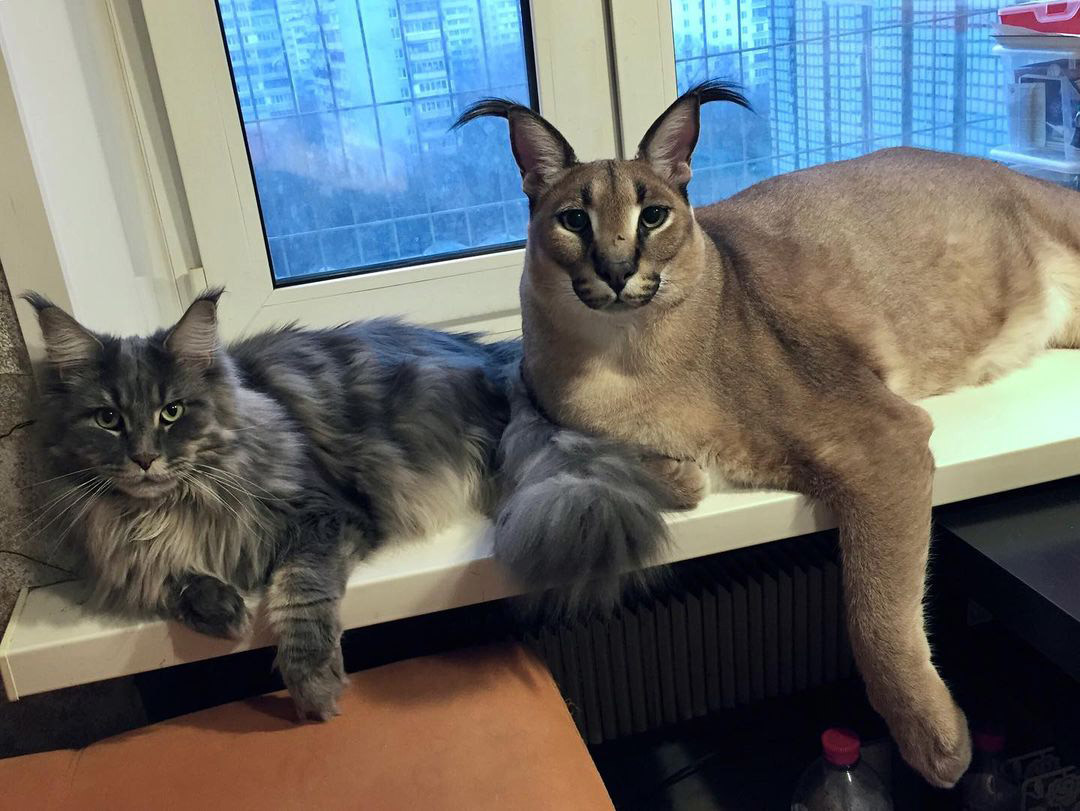
\includegraphics[width=\linewidth]{img/60b4cf3885600a50dd341bb2.jpg}
\end{frame}

\begin{frame}
    \frametitle{Evaluation}

    \begin{itemize}
        \item \emph{Production and Marketability} The system is working, but not very well tested. For production use, we require more usability tests, readily-set-up node boards etc.. Possibly ones with multiple pumps. (Like the other group did.)
        \item \emph{Network Usage}
        \item \emph{Storage Usage} The table with the most entries will most likely be the \texttt{plant\_humidities} table. Given one node, one entry in the table could be made up from a single byte for the node id (for the \texttt{plant\_nodes} table), up to eight bytes for the timestamp and one 16 bit humidity value. So in a day, given that we send one value every five seconds, we might store up to \((1+8+2) \cdot (24 \cdot 60 \cdot 60) / 5 = 19008\) bytes, so about \(5702400\) bytes (\(\approx 6\)MB) in a 30-day-month.
    \end{itemize}
\end{frame}

\begin{frame}
    \frametitle{Evaluation}
    \begin{itemize}
        \item \emph{Energy Usage} Some factors that influence the reproducibility of our result:
        \item \emph{Scalability and Availability Measures} For more nodes, one can easily allow more DTLS sessions to be added to the proxy. In the frontend we took care of some edge cases which could result in a slow service, like not requesting all data from the database when we want to build the humidity graph. Given a strong enough host, we claim that up to a hundred devices can safely be handled by the system. (Which may seem ridiculous, but it might yield an interesting discussion.)
    \end{itemize}
\end{frame}

\begin{frame}{Software Development Practices}
    We deployed:
    \begin{itemize}
        \item Agile development with Kanban
        \item Versioning and Branching with git
        \item Communication with Discord
        \item Splitting up in several groups and performing integration tests
        \item Regularly writing minimal documentation
        \item Code Conventions
        \item Static Code Analysis
    \end{itemize}
    And some more techniques.
\end{frame}

\begin{frame}{Reflecting on our Work}
    The development was rather rough.
    \begin{itemize}
        \item Lack of documentation for specific parts, such as the humidity sensor. We are no electric engineers, despite our best efforts, and do not know all the small tricks.
        \item Initial hardware was simply failing. In our report, we outline how we tried to build a small circuit for connecting the pump, but a faulty transistor deminished our efforts.
        \item Despite our best efforts of communicating changes on different parts and how they effect others, this still lead to some systems not working. E.g. when the DTLS proxy was developed, a false commit broke communication on another branch as DTLS there was enabled, but proxy was not yet functional.
    \end{itemize}

    Despite that, the system is working and mainly employs secure and standardized, open technologies.
\end{frame}

\begin{frame}{Possible Future Enhancements (\emph{Some} Ideas, there are Lots)}
    \begin{itemize}
        \item \texttt{hw}: A case for the controllers and their circuitry.
        \item \texttt{front}: TypeScript instead of JavaScript, use HTTP/2.0 or even 3.0 over QUIC.
        \item \texttt{proxy}: Better RNG for \texttt{tinydtls} and multiple possible improvements to the proxy, see \texttt{README.md}
    \end{itemize}

    And more, see the repository.
\end{frame}

\end{document}
